\section{Versuchsaufbau}
\label{versuchsaufbau}

Generelle Netzstruktur, softmax auf Klassen abgebildet
Conv mit MaxPool gefolgt von AveragePool auf Fully Connect auf Softmax

wir machen hier nur klassifikation
ander probleme sind aber denkbar (z.B. Segmentierung über Knotenklassifizierung)

\subsection{Datensätze}
\label{datensaetze}

Die vorgestellten Faltungsmethoden aus Kapitel~\ref{raeumliches_lernen} und~\ref{spektrales_lernen} \bzgl{} des Lernens auf Graphen im zweidimensionalen euklidischen Raum werden über einer Reihe von Datensätzen verifiziert, die im Folgenden vorgestellt werden.
Dafür werden die Bildermengen in eine Superpixelrepräsentation (\gls{SLIC} und Quickshift) konvertiert und darauf basierend in eine Graphrepräsentation transformiert (\vgl{} Kapitel~\ref{graphrepraesentationen_von_bildern}).
Zusätzlich zu der Präsentation der Datensätze enthält dieses Unterkapitel damit insbesondere die Parameterwahl der jeweiligen Superpixelalgorithmen, welche jeweils händisch über einer Untermenge der Bilder eines jeden Datensatzes ermittelt werden.
Weiterhin wird in diesem Unterkapitel abhängig von dem gewählten Datensatz und der Superpixelrepräsentation auf die entsprechenden Merkmalsselektionen der $38$ Formmerkmale eingegangen, die nach dem beschriebenen Prinzip aus Kapitel~\ref{merkmalsselektion} errechnet werden.

\paragraph{MNIST}
\label{mnist}

Der \emph{\gls{MNIST}} Datensatz enthält eine große Menge eindeutig klassifizierter handgeschriebener Zahlen von $0$ bis $9$, welcher daher zum Lernen einer Schrift- \bzw{} Zahlenerkennung genutzt werden kann~\cite{mnist}.
Er besteht aus $55000$ Trainingsbildern, $5000$ Validierungsbildern sowie $10000$ Testbildern.
Die Bilder des Datensatzes sind einheitlich auf die Größe $28 \times 28$ skaliert und besitzen lediglich einen Farbkanal mit Grauwerten, welcher angibt, ob ein Pixel des Bildes zu einer Zahl (weiß), zu deren Rand oder zum Hintergrund (schwarz) gehört~\cite{mnist}.
Aufgrund seiner kleinen Datengröße und leichten Handhabung gilt er als die ideale Einführung in Prinzipien des maschinellen Lernens und zeichnet sich damit als ideal für die Verifizierung eines neuen Ansatzes \bzgl{} neuronaler Netze aus.
Insbesondere kann der Datensatz während des gesamten Trainings im Hauptspeicher gehalten werden, was den Aufwand \bzgl{} der Verarbeitung und Eingabe der Daten auf ein Minimum reduziert.

Die ermittelten Parameter \bzgl{} der beiden benutzten Superpixelalgorithmen sind in Tabelle~\ref{tab:mnist} gegeben.
Für \gls{SLIC} sind das die Parameter $K \in \gls{N}$, \dhe{} die Anzahl der gewünschten Segmente, sowie $F \in \gls{R}$ für die Gewichtung zwischen der Form und den Farbabgrenzungen der Superpixel.
Für Quickshift ergeben sich dagegen drei wählbare Parameter — $\gls{sigma} \in \gls{R}$ für die Wahl der Standardabweichung der Gaußfunktion, $\alpha \in \gls{R}$ für die Gewichtung des Farbterms sowie $S \in \gls{N}$ zur Einschränkung der Berechnung über ein Fenster der Größe $S \times S$.
Für eine detaillierte Beschreibung der Parameter sei auf Kapitel~\ref{superpixel_verfahren} verwiesen.
\begin{table}[t]
\centering
\begin{tabular}{rlrlrlrlrlrl}
  \toprule
  \multicolumn{6}{c}{\gls{SLIC}} & \multicolumn{6}{c}{Quickshift}\\
  \midrule
  $K$ & $100$ & $F$ & $5$ & & & $\gls{sigma}$ & $2$ & $\alpha$ & $1$ & $S$ & $2$\\
  \midrule
  $\overline{N}$ & $64.6$ & $N_{\min}$ & $50$ & $N_{\max}$ & $80$ & $\overline{N}$ & $82.1$ & $N_{\min}$ & $5$ & $N_{\max}$ & $154$\\
  $\overline{\gls{degree}}$ & $5.7$ & $\gls{degree}_{\min}$ & $1$ & $\gls{degree}_{\max}$ & $19$ & $\overline{\gls{degree}}$ & $6.8$ & $\gls{degree}_{\min}$ & $1$ & $\gls{degree}_{\max}$ & $101$\\
  \bottomrule
\end{tabular}
\caption[\gls{MNIST} Superpixelparameter]{Wahl der Superpixelparameter des \gls{MNIST} Datensatzes.}
\label{tab:mnist}
\end{table}

Aus der Wahl der Superpixelparameter ergeben sich die ebenfalls in der Tabelle datierten Werte der durchschnittlichen, minimalen und maximalen Anzahl an Knoten $\overline{N}$, $N_{\min}$ \bzw{} $N_{\max}$ sowie dem durchschnittlichen, minimalen und maximalen Knotengrad $\overline{\gls{degree}}$, $\gls{degree}_{\min}$ \bzw{} $\gls{degree}_{\max}$ über der Menge aller aus den Bildern generierten Graphen bei einer Konnektivität von $8$.
Wohingegen \gls{SLIC} über alle Bilder relativ gleich große Knotenmengen mit relativ gleichem Knotengrad erzeugt, kann dies bei Quickshift je nach Bild stark variieren.
So erzeugt Quickshift in dem \gls{MNIST} Datensatz \bspw{} große schwarze Bereiche für den Hintergrund, die dementsprechend auch einen sehr hohen Knotengrad besitzen.
Bei \gls{SLIC} werden stattdessen auch die gleichfarbigen, schwarzen Flächen in einheitliche Intervalle unterteilt.
Abbildung~\ref{fig:mnist} veranschaulicht die beiden Superpixel- \bzw{} Graphrepräsentationen anhand eines Bildes aus dem \gls{MNIST} Datensatz.
\section{MNIST}

Trainingsbilder: 55.000

\begin{itemize}
  \item 10.000 Steps mit Batch Size 64 (ungefähr 12 Epochen)
  \item Learning Rate 0.001
  \item klassisches Convolution Neural Network nachgebildet mit Gridgraphen
  \item Conv1: $5 \times 5$, $1 \rightarrow 32$
  \item MaxPool1: Size 2, Stride 2
  \item Conv2: $5 \times 5$, $32 \rightarrow 64$
  \item MaxPool2: Size 2, Stride 2
  \item FC1: 1024
  \item Dropout: 0.5
  \item FC2: 10
\end{itemize}

\subsection{Auswertung}

\begin{itemize}
  \item \textbf{2D Conv > Max:} 0.18s pro Batch, Accuracy: 99.189, Cost: 0.03458
  \item \textbf{2D Conv > 2D Conv > Max:} 0.25s pro Batch, Accuracy: 99.139, Cost: 0.03062
  \item \textbf{Chebyshev $k=25$ GCNN:} 0.91s pro Batch, Accuracy: 98.888, Cost: 0.04329
  \item \textbf{$k=1$ GCNN:} 0.22s pro Batch, Accuracy: 96.765, Cost: 0.10596
  \item \textbf{Partitioned GCNN:}
  \begin{itemize}
    \item Conv > Max: 0.45s pro Batch, Accuracy: 98.998, Cost: 0.03198
    \item Conv > Conv > Max: 2.87s pro Batch, Accuracy: 99.189, Cost: 0.02704
  \end{itemize}
\end{itemize}

\subsection{SLIC}

\begin{itemize}
  \item keine lokale Normierung
  \item Stddev: $1$
  \item 4 Level
  \item Graphkonnektivität: $1$
  \item Anzahl Segmente: $100$
  \item Compactness: $10$
  \item Maximum Iterations: $10$
  \item Sigma: $0$
  \item Anzahl Partitionen: 8
  \item Features: Area, Bbox height, bbox width, Mean Color = $4$ Features
  \item \textbf{Aufbau}: Conv zu 32, Pool2, Conv zu 64, Pool2, Conv zu 128, Pool2, Conv zu 256, Pool2, AveragePool, FC210
  \item Meiste zeit wird durch Partitionierung verschwendet.
  \item \textbf{Ergebnisse}: 0.79s pro Batch, Accuracy: 0,79497, Loss: 0.62814
  \item enttäuschend!
\end{itemize}

\section{PascalVOC}

erster Test:
17 s Preprocess, 12s Training auf BatchSize 64
loss = 0.2, acc = 0.55


Die in Kapitel~\ref{merkmalsselektion} beschriebene Merkmalsselektion reduziert für \gls{MNIST} die Menge an Formmerkmalen (\vgl{} Kapitel~\ref{merkmalsextraktion}) im ersten statistisch basierten Test auf $12$ Merkmale, welche im zweiten Schritt rekursiv auf $9$ Merkmale reduziert werden.
Die ermittelten (unterschiedlichen) Formmerkmale für \gls{SLIC} und Quickshift \bzgl{} \gls{MNIST} sind in Tabelle~\ref{tab:mnist_merkmale} aufgezeigt.
\begin{table}[t]
\centering
\begin{tabular}{lccccccccc}
  \toprule
  \gls{SLIC} & $\hat{x}$ & $\hat{y}$ & $\mathrm{ecc}$ & $\mathrm{dia}$ & $\mathrm{ext}$ & $\gls{mu}^{\prime}_{20}$ & $\gls{lambda}_2$ & $\mathrm{axis}_1$ & $\mathrm{axis}_2$\\
  Quickshift & $\hat{x}$ & $\mathrm{ecc}$ & $\mathrm{dia}$ & $\mathrm{ext}$ & $\gls{mu}_{03}$ & $\gls{mu}_{21}$ & $\gls{mu}_{30}$ & $\gls{eta}_{03}$ & $\mathrm{ori}$\\
  \bottomrule
\end{tabular}
  \caption[\gls{MNIST} Merkmalsselektion]{Merkmalsselektion des \gls{MNIST} Datensatzes zu $9$ Formmerkmalen.}
\label{tab:mnist_merkmale}
\end{table}
Wohingegen sich die Merkmalsselektion bei \gls{SLIC} eher für Formmerkmale entscheidet, die aus den Momenten gewonnen werden können, genießen bei Quickshift die reinen translationsinvarianten Momente \gls{mu} ein größeres Interesse.
Daraus ergeben sich $10$ Merkmale eines Knotens inklusive der Durchschnittsfarbe eines Superpixels.

\paragraph{CIFAR-10}
\label{cifar_10}

Der \emph{\gls{Cifar}} Datensatz, auch \gls{Cifar}-10 genannt, besteht aus $60000$ farbigen Bildern, die jeweils genau einer von $10$ Klassen zugeordnet sind~\cite{cifar_10}.
$45000$ Bilder werden dabei als Trainingsbilder, $5000$ als Validierungsbilder und $10000$ als Testbilder genutzt.
Zu jeder Klasse existieren genau $6000$ Bilder, welche gleichmäßig auf die Bilduntermengen aufgeteilt sind.
Die Klassen der Bilder sind im Folgenden: Flugzeug, Auto, Vogel, Katze, Reh, Hund, Frosch, Pferd, Schiff und Lastwagen.
Die Bilder der Klassen sind dabei \emph{einander ausschließend}.
So enthält die Klasse \enquote{Auto} nur kleinere Personenwagen, wohingegen die Klasse \enquote{Lastwagen} auch nur als solche zu klassifizierenden Fahrzeuge enthält~\cite{cifar_10}.
Die Bilder haben eine einheitliche Größe von $32 \times 32$ Pixeln und besitzen drei Farbkanäle.
Sie passen aufgrund ihrer Größe ähnlich zu \gls{MNIST} komplett in den Hauptspeicher.
Aufgrund dessen ist er für eine Bildklassifizierung sehr beliebt, da er schnelle Trainingszeiten garantiert und dabei trotzdem alle Techniken des Deep Learnings ausgeschöpft werden müssen, um qualitativ hochwertige Resultate zu erzielen.
Der \gls{Cifar} Datensatz liegt ebenfalls in einer zweiten Version vor, genannt \gls{Cifar}-100, der 60000 Bilder in 100 Klassen unterteilt, welcher aber in dieser Arbeit keine Verwendung findet~\cite{cifar_10}.

Tabelle~\ref{tab:cifar_10} zeigt die Wahl der Parameter der beiden Superpixelalgorithmen.
\begin{table}[t]
\centering
\resizebox{\textwidth}{!}{%
\begin{tabular}{rlrlrlrlrlrl}
  \toprule
  \multicolumn{6}{c}{\gls{SLIC}} & \multicolumn{6}{c}{Quickshift}\\
  \midrule
  $K$ & $200$ & $F$ & $5$ & & & $\gls{sigma}$ & $1$ & $\alpha$ & $1$ & $S$ & $5$\\
  \midrule
  $\overline{N}$ & $232.1$ & $N_{\min}$ & $186$ & $N_{\max}$ & $263$ & $\overline{N}$ & $182.0$ & $N_{\min}$ & $18$ & $N_{\max}$ & $624$\\
  $\overline{\gls{degree}}$ & $6.3$ & $\gls{degree}_{\min}$ & $1$ & $\gls{degree}_{\max}$ & $21$ & $\overline{\gls{degree}}$ & $7.4$ & $\gls{degree}_{\min}$ & $1$ & $\gls{degree}_{\max}$ & $67$\\
  \bottomrule
\end{tabular}}
\caption[\gls{Cifar}-10 Superpixelparameter]{Wahl der Superpixelparameter des \gls{Cifar}-10 Datensatzes.}
\label{tab:cifar_10}
\end{table}
Im Vergleich zu dem \gls{MNIST} Datensatz würden dafür insbesondere für \gls{SLIC} die approximierte Anzahl an Superpixeln von 100 auf 200 und für Quickshift die Größe des Fensters $S$ von 2 auf 5 erhöht.
Weiterhin zeigt die Tabelle erneut Informationen zu den generierten Graphen über die Anzahl der Knoten und ihrer Knotengraden.
Hier lassen sich ebenfalls wieder die unterschiedlichen Vorgehensweisen der beiden Superpixelalgorithmen erkennen.
Die maximale Anzahl an Knoten eines Graphen aus der Quickshift-Segmentierung liegt dabei mit $624$ Knoten sehr hoch, \dhe{} im Durchschnitt werden nur zwei Pixel einem Superpixel zugeordnet werden, und kann als extremer Ausreißer gewertet werden.
Abbildung~\ref{fig:cifar_10} zeigt ein Bildes des \gls{Cifar}-10 Datensatzes mit dessen entsprechenden Superpixel- \bzw{} Graphrepräsentationen.
\begin{figure}[t]
\centering
\subfigure[\gls{SLIC}]{%
  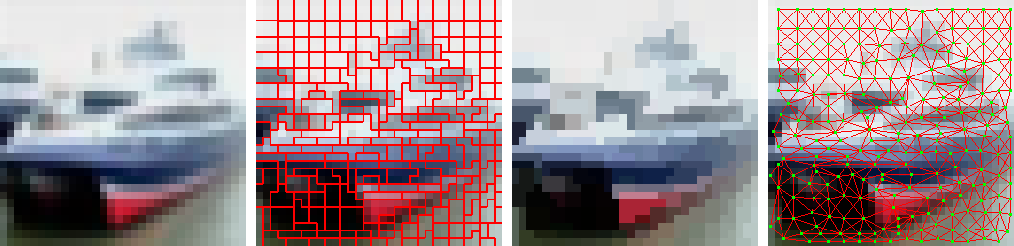
\includegraphics[width=\textwidth]{bilder/cifar_10_slic.png}
}
\subfigure[Quickshift]{%
  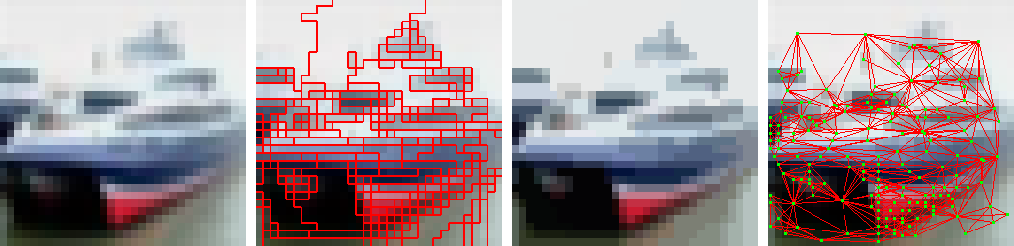
\includegraphics[width=\textwidth]{bilder/cifar_10_quickshift.png}
}
  \caption[\gls{Cifar}-10]{Bild des \gls{Cifar}-10 Datensatzes~\cite{cifar_10}, jeweils dargestellt als (1) Originalbild, (2) Superpixelrepräsentation, (3) Durchschnittsfarbe der Superpixel und (4) Graphrepräsentation.}
\label{fig:cifar_10}
\end{figure}


Analog zu \gls{MNIST} wurden für den \gls{Cifar}-10 Datensatz erneut $9$ Formmerkmale nach dem gleichen Prinzip ermittelt.
Tabelle~\ref{tab:cifar_10_merkmale} zeigt die berechnete Wahl der Merkmale der Selektion.
\begin{table}[t]
\centering
\begin{tabular}{lccccccccc}
  \toprule
  \gls{SLIC} & $\gls{M}_{00}$ & $\mathrm{box}_y$ & $\hat x$ & $\mathrm{dia}$ & $\mathrm{ext}$ & $\gls{hu}_1$ & $\gls{lambda}_1$ & $\mathrm{axis}_1$ & $\mathrm{axis}_2$\\
  Quickshift & $\mathrm{box}_y$ & $\mathrm{box}_x$ & $\hat x$ & $\hat y$ & $\mathrm{ecc}$ & $\mathrm{ext}$ & $\gls{lambda}_1$ & $\mathrm{axis}_1$ & $\mathrm{axis}_1$\\
  \bottomrule
\end{tabular}
  \caption[\gls{Cifar}-10 Merkmalsselektion]{Merkmalsselektion des \gls{Cifar}-10 Datensatzes zu $9$ Formmerkmalen.}
\label{tab:cifar_10_merkmale}
\end{table}
Es ist auffällig, dass sich für die beiden Superpixelrepräsentation dabei die Selektion der Merkmale bei nur drei von neun Merkmalen unterscheidet.
Inklusive den Durchschnittsfarbwerten eines Superpixels über den drei Farbkanälen ergeben sich daraus jeweils $12$ Knotenmerkmale.
Bei einer durchschnittlichen Anzahl an Knoten von $232.1$ bei \gls{SLIC} \bzw{} von $182.0$ bei Quickshift führt dies zu einer Berechnung von $2785$ \bzw{} $2184$ Merkmalen eines Graphen.
Im Vergleich zu der Anzahl an Merkmalen des Originalbildes $\left(32 \times 32 \times 3 = 3072\right)$ ergibt sich folglich eine Datenreduktion von $9.34\%$ \bzw{} $28.91\%$.
Das ist aufgrund der ursprünglichen Bildgrößen des \gls{Cifar}-10 Datensatzes eine nicht zu unterschätzende Datenreduktion, bei der kaum entscheidende Informationen des Bildes verloren gehen (\vgl{} Abbildung~\ref{fig:cifar_10}).

\paragraph{PASCAL VOC}
\label{pascal_voc}

Der \emph{\gls{Pascal}} Datensatz besteht aus $17126$ farbigen Bildern beliebiger Größen, der aufgrund seiner ausführlichen Bildannotierungen nicht nur für eine Bildklassifizierung, sondern ebenfalls für Objektdetektionen oder eine Bildsegmentierung genutzt werden kann~\cite{pascal_voc}.
Zu jedem Bild stehen insbesondere Informationen zu den enhaltenden Objekten und deren Hüllkörpern zur Verfügung~\cite{pascal_voc}.
Ein Bild besitzt dabei minimal ein Objekt der $20$ annotierten Objektklassen.
Gleiche oder unterschiedliche Objektklassen können mehrfach in einem Bild existieren.
Die enthaltenden Objekte der Bilder sind im Einzelnen~\cite{pascal_voc}:
\begin{itemize}
  \item Person
  \item Vogel, Katze, Kuh, Hund, Pferd, Schaf
  \item Flugzeug, Fahrrad, Boot, Bus, Auto, Motorrad, Zug
  \item Flasche, Stuhl, Esstisch, Topfblume, Sofa, Fernseher/Monitor
\end{itemize}
Die Höhen und Breiten der Bilder reichen von von $142$ bis $500$ Pixeln.
Die durchschnittliche Bildgröße des Datensatzes beträgt $389 \times 467$ Pixel und ist damit um einiges größer als der zuvor betrachtete \gls{Cifar}-10 Datensatz.

\gls{Pascal} besitzt keine eindeutige Zuordnung der Bilder in Trainings-, Validierungs und Testbildern.
Es existiert zwar ein seperator Testdatensatz, jedoch stehen dessen Annotierungen nicht zur freien Verfügung.
Folglich wird aus der Bildermenge zufällig eine Validierungs- \bzw{} Testmenge von $1500$ Bildern generiert.
Damit stehen noch $15626$ Bilder für das Training eines neuronalen Netzes zur Verfügung.



\begin{table}[t]
\centering
\resizebox{\textwidth}{!}{%
\begin{tabular}{rlrlrlrlrlrl}
  \toprule
  \multicolumn{6}{c}{\gls{SLIC}} & \multicolumn{6}{c}{Quickshift}\\
  \midrule
  $K$ & $1600$ & $F$ & $30$ & & & $\gls{sigma}$ & $2$ & $\alpha$ & $0.75$ & $S$ & $8$\\
  \midrule
  $\overline{N}$ & $1540.9$ & $N_{\min}$ & $1082$ & $N_{\max}$ & $1839$ & $\overline{N}$ & $2131.6$ & $N_{\min}$ & $234$ & $N_{\max}$ & $29010$\\
  $\overline{\gls{degree}}$ & $6.5$ & $\gls{degree}_{\min}$ & $1$ & $\gls{degree}_{\max}$ & $50$ & $\overline{\gls{degree}}$ & $7.7$ & $\gls{degree}_{\min}$ & $1$ & $\gls{degree}_{\max}$ & $256$\\
  \bottomrule
\end{tabular}}
\caption[\gls{Pascal} Superpixelparameter]{Wahl der Superpixelparameter des \gls{Pascal} Datensatzes.}
\label{tab:pascal_voc}
\end{table}

\begin{figure}[t]
\centering
\subfigure[\gls{SLIC}]{%
  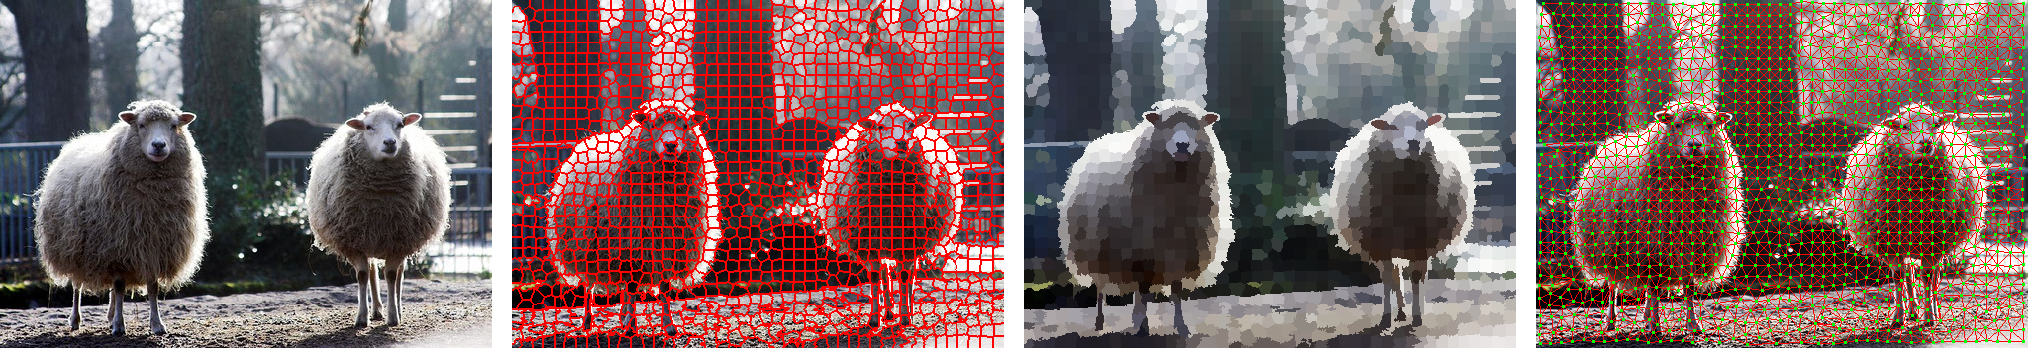
\includegraphics[width=\textwidth]{bilder/pascal_voc_slic.png}
}
\subfigure[Quickshift]{%
  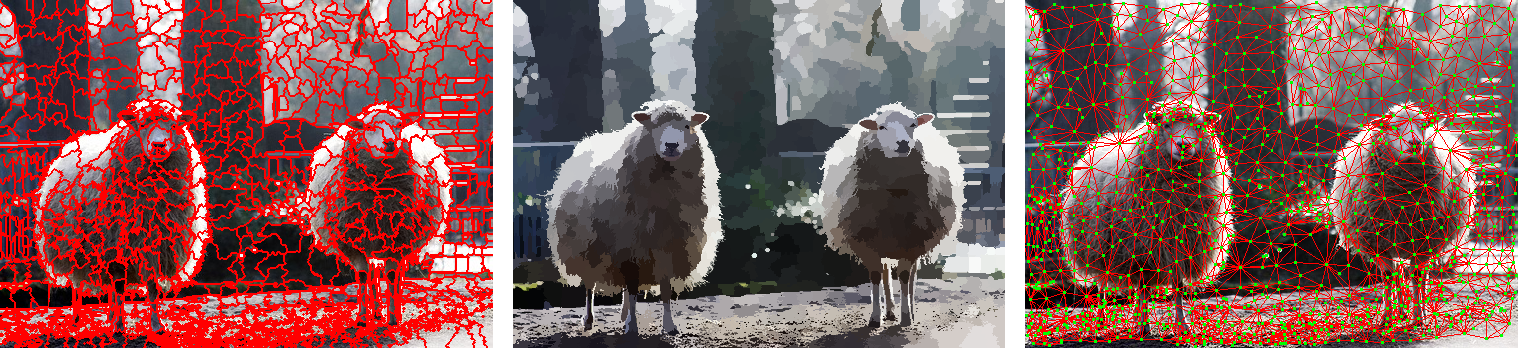
\includegraphics[width=\textwidth]{bilder/pascal_voc_quickshift.png}
}
  \caption[\gls{Pascal}]{Bild des \gls{Pascal} Datensatzes~\cite{pascal_voc}, jeweils dargestellt als (1) Originalbild, (2) Superpixelrepräsentation, (3) Durchschnittsfarbe der Superpixel und (4) generierter Graph.}
\label{fig:pascal_voc}
\end{figure}


datenreduktion

\paragraph{Weitere Datensätze}
\label{weitere_datensaetze}

\subsection{Metriken}
\label{metriken}

Loss Function
Accuracy

\subsection{Parameterwahl}
\label{parameterwahl}

Vorstellung aller Parameter
Was gibt es denn hier überhaupt?
Dropout, L2 Regularisierung?
BatchSize?
Globale/normale Lokalisierung
Standardabweichung für Gauß
LEARNING RATE, LEARNING RATE DECAY

Alle Faltungen wurden dabei mit einer Partitionsgröße von $8$ bei $K=0$ und $K=1$ implementiert, um ein \gls{CNN} mit einem $3 \times 3$ Filter zu simulieren.
Es erscheint jedoch vorstellbar die Filtergröße bei größerer lokaler Kontrollierbarkeit, \dhe{} $K > 1$, weiter zu reduzieren und die Gefahr des Overfittings damit aufgrund der kleineren Anzahl an Trainingsparametern einzuschränken.

\paragraph{Datenreduktion}
\label{datenreduktion}

\subsection{Augmentierung von Graphen}
\label{augmentierung_von_graphen}

hier auf die Formeln von TensorFlow referenzieren, d.h. TensorFlow Quelle angeben
\cite{tensorflow}

Augmentierung auf Graphen über left/right
Farbanpassungen


nesser ist es, dass Bild vorher zu ändern, da sich dadurch die Superpixelrepräsentation ändert
und folglich zu realisiterischer Augmentierung führt.

\subsection{Vorverarbeitung und Eingabe der Daten}
\label{vorverarbeitung}
